%%%%%%%%%%%%%%%%%%%%%%%%%%%%%%%%%%%%%%%%%%%%%%%%%%%%%%%%%%%%%%%%%%%%%%%%%%%%%%%%
% Copyright 2023 Louis Paternault --- http://snt.ababsurdo.fr
%
% Publi� sous licence Creative Commons Attribution-ShareAlike 4.0 International (CC BY-SA 4.0)
% http://creativecommons.org/licenses/by-sa/4.0/deed.fr
%%%%%%%%%%%%%%%%%%%%%%%%%%%%%%%%%%%%%%%%%%%%%%%%%%%%%%%%%%%%%%%%%%%%%%%%%%%%%%%%

% Pour compiler :
%$ lualatex $basename

\documentclass[tikz]{standalone}

\usetikzlibrary{arrows, automata, positioning}

\begin{document}
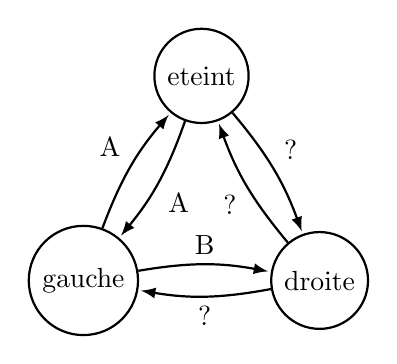
\begin{tikzpicture}[shorten >=1pt, auto, thick, scale=1.5]
\tikzstyle{everry state}=[minimum width={width("gauche")},inner sep=1pt]
\node[state] (eteint) at (0, {sqrt(3)}) {eteint};
\node[state] (gauche) at (-1, 0) {gauche};
\node[state] (droite) at (1, 0) {droite};

\path[-latex]
   (eteint) edge[bend left=10] node{A} (gauche)
            edge[bend left=10] node{?} (droite)
    (gauche) edge[bend left=10] node{A} (eteint)
             edge[bend left=10] node{B} (droite)
    (droite) edge[bend left=10] node{?} (eteint)
             edge[bend left=10] node{?} (gauche)
	 ;
\end{tikzpicture}
\end{document}
